% =============================================================================
%  manuscript.tex
%  Draft submission to Computers & Geosciences (Elsevier)
%
%  Compile from this directory:
%      ./compile.sh manuscript.tex
% =============================================================================

% --- elsarticle alternative (uncomment when ready to submit) -----------------
% \documentclass[review,12pt,authoryear]{elsarticle}
% \journal{Computers \& Geosciences}
% -----------------------------------------------------------------------------
\documentclass[11pt,a4paper]{article}

\usepackage[a4paper,margin=2.5cm]{geometry}
\usepackage{lineno}
\usepackage[colorlinks=true,linkcolor=blue!50!black,citecolor=blue!40!black,urlcolor=blue!50!black]{hyperref}
\usepackage{graphicx}
\usepackage{amsmath,amssymb}
\usepackage{booktabs}
\usepackage{xcolor}
\usepackage{listings}
\usepackage{enumitem}
\usepackage{microtype}
\usepackage{authblk}
\usepackage[super,sort&compress]{natbib}
\usepackage{algorithm}
\usepackage{algpseudocode}
\usepackage{dblfloatfix}   % allow figure*/table* at the bottom of a page
\usepackage{quantikz}
\usepackage{makecell}
\usepackage{tikz}
\usetikzlibrary{arrows.meta, fit, backgrounds, shapes.geometric}

% Looser float-placement parameters so figures don't get pushed pages away.
\renewcommand{\topfraction}{0.95}
\renewcommand{\bottomfraction}{0.95}
\renewcommand{\textfraction}{0.05}
\renewcommand{\floatpagefraction}{0.7}
\renewcommand{\dbltopfraction}{0.95}
\renewcommand{\dblfloatpagefraction}{0.7}
\setcounter{topnumber}{3}
\setcounter{bottomnumber}{3}
\setcounter{totalnumber}{6}
\setcounter{dbltopnumber}{3}

\renewcommand{\Authfont}{\bfseries}
\renewcommand{\Affilfont}{\mdseries\normalfont\small}
\setlength{\affilsep}{0.4em}

\modulolinenumbers[5]

% Expose the internal @twocolumnfalse environment so the title/abstract can
% span both columns via \twocolumn[\begin{strip}...\end{strip}].
\makeatletter
\newenvironment{strip}{\begin{@twocolumnfalse}}{\end{@twocolumnfalse}}
\makeatother

\definecolor{todoRed}{RGB}{180,30,30}
\newcommand{\todonote}[1]{\textcolor{todoRed}{\textbf{[TODO: #1]}}}
\newcommand{\needs}[1]{\textcolor{todoRed}{\textbf{[NEEDED: #1]}}}
% Mark newly-introduced citations so the author can vet them against the
% curated refs.bib.  Usage: \newcite{Smith2020}.
\newcommand{\newcite}[1]{\textcolor{todoRed}{$^{\ast}$}\citep{#1}}

% Drop-in replacements for elsarticle's frontmatter / highlights / keyword envs
\newenvironment{frontmatter}{}{}
\newenvironment{highlights}{%
  \begin{quote}\textbf{Highlights}\par\vspace{-0.5em}
  \begin{itemize}[leftmargin=2em,itemsep=0pt]%
}{%
  \end{itemize}\end{quote}%
}
\newenvironment{keyword}{%
  \par\noindent\textbf{Keywords:}\;%
}{\par\medskip}
\providecommand{\sep}{,\ }

\lstset{
  basicstyle=\ttfamily\footnotesize,
  breaklines=true,
  frame=single,
  language=Python,
  showstringspaces=false,
}

\title{Accelerating full waveform inversion using hybrid quantum-classical finite basis physics-informed neural networks}

\author[a,*]{Hoang Anh Nguyen}
\author[b]{Divakar Vashisth}
\author[a]{Ali Tura}
\affil[a]{Department of Geophysics, Colorado School of Mines, Golden, CO 80401, USA}
\affil[b]{Department of Energy Science and Engineering, Stanford University, Stanford, CA 94305,USA}
\affil[*]{Corresponding author: \href{mailto:hoanganh_nguyen@mines.edu}{hoanganh\_nguyen@mines.edu}}

\date{\today}

\begin{document}

\maketitle

% =============================================================================
%  FRONT MATTER
% =============================================================================
\begin{frontmatter}

% --- Abstract ----------------------------------------------------------------
\begin{abstract}
Full waveform inversion (FWI) reconstructs subsurface material properties from seismic data but remains computationally demanding. Physics-informed neural networks (PINNs) and their domain-decomposed variants (FBPINNs) offer a mesh-free alternative but face convergence challenges when representing complex velocity fields. We present a hybrid quantum-classical FBPINN for acoustic FWI, in which the velocity network is implemented as a classical-to-quantum pipeline terminating in a parameterized quantum circuit (PQC). The PQC is realized as a differentiable JAX statevector simulator, enabling end-to-end automatic differentiation through the classical PINN, the quantum circuit, and the physics-informed loss. On a laterally-varying velocity benchmark, the quantum hybrid reaches a lower L1 velocity error than a classical FBPINN baseline in approximately $8\times$ fewer training iterations, using $\sim$$33$\% fewer trainable parameters, and outperforms all 15 classical hyperparameter variants tested. A second benchmark (checkerboard) demonstrates the generality of the inversion pipeline; quantum hybrid results for that benchmark are forthcoming. Our framework is broadly applicable to wave-based inverse problems beyond geophysics, including medical ultrasound tomography and non-destructive evaluation.
\end{abstract}

% --- Keywords ----------------------------------------------------------------
\begin{keyword}
FWI, Seismic, Wave Propagation, Quantum Computing, Parameterized Quantum Circuit, PINNs
\end{keyword}

\end{frontmatter}

\linenumbers

% =============================================================================
% Paper Body
% =============================================================================

\section{Introduction}

Full Waveform Inversion (FWI) is a powerful technique for reconstructing material properties from recorded waveform data by exploiting the full information content of wave signals, including amplitude, phase, and frequency. Originally developed in the context of exploration geophysics for subsurface velocity imaging \citep{Tarantola1984}, FWI has since become central to a wide range of disciplines. In seismology, it enables high-resolution imaging of crustal and mantle structures \citep{Fichtner2009, Ebru2011}, and is increasingly applied to high-density datasets acquired via distributed acoustic sensing (DAS) \newcite{Zhan2020}; in hydrocarbon exploration, it provides detailed velocity models for reservoir characterization \citep{Virieux2009}. Beyond geophysics, FWI principles have found growing applications in medical imaging, where ultrasound computed tomography employs waveform inversion to reconstruct tissue properties for breast cancer detection and characterization \citep{10.1121/1.3699240, Sandhu_2015}, and in photoacoustic tomography, where wave-based inversion recovers optical absorption maps from acoustic measurements \citep{Wang2016}. Non-destructive evaluation of engineering structures similarly leverages full waveform methods to detect defects and characterize material properties \citep{7422116}. Despite its versatility across these domains, FWI remains computationally demanding, requiring iterative solutions of the forward wave equation and the computation of gradients through adjoint-state methods, often at substantial cost for large-scale and high-frequency problems.

Physics-Informed Neural Networks (PINNs) have emerged as a mesh-free alternative for solving partial differential equations (PDEs), embedding the governing physics directly into the loss function of a neural network \citep{RAISSI2019686}. By minimizing residuals of the PDE at collocation points, PINNs approximate solutions without traditional numerical discretization. This paradigm has been extended to inverse problems, where unknown model parameters, such as the velocity and density fields in FWI, are jointly optimized alongside the wavefield solution. Recent works have applied PINNs to wave-related problems, including solving the wave equation in the frequency domain \citep{10.1093/gji/ggab010}, seismic traveltime tomography \citep{waheed2021pinntomoseismictomographyusing}, and medical imaging applications \citep{10230537}, offering a fundamentally different approach to the classical adjoint-state framework. In particular, \citep{rahst} demonstrated the application of PINNs to FWI, achieving accurate velocity reconstruction from seismic data by jointly optimizing wavefield and velocity network parameters. However, standard PINNs face well-documented challenges when applied to problems involving high-frequency wave propagation, multi-scale physics, and large computational domains. The spectral bias of neural networks, their tendency to learn low-frequency features before high-frequency ones, can severely limit convergence in wave propagation problems. To address these limitations, Finite Basis Physics-Informed Neural Networks (FBPINNs) were introduced by \citet{Moseley2023}, employing a domain decomposition strategy in which the global solution is represented as a sum of locally supported basis functions, each parameterized by an independent neural network. This approach effectively mitigates spectral bias, improves parallel scalability, and enables the solution of problems that are intractable for standard PINNs.  To date, no work has combined the domain decomposition advantages of FBPINNs for waveform inversion.

In parallel with advances in scientific machine learning, quantum computing has attracted growing interest for its potential to accelerate computational tasks across diverse domains. Parameterized Quantum Circuits (PQCs), also known as variational quantum circuits, have emerged as a near-term approach to quantum machine learning, operating within the constraints of current Noisy Intermediate-Scale Quantum (NISQ) devices \citep{Preskill2018quantumcomputingin}. PQCs encode classical data into quantum states through feature maps, process the information through parameterized unitary operations, and extract classical outputs via measurement. Several studies have explored the integration of quantum circuits with neural networks, forming hybrid quantum-classical architectures that leverage the expressive power of quantum Hilbert spaces while maintaining the trainability and flexibility of classical networks \citep{PhysRevA.101.032308, Benedetti_2019, Ostaszewski2021structure}.

The intersection of quantum computing and PINNs has begun to receive attention, with recent works investigating Quantum Physics-Informed Neural Networks (QPINNs) for solving differential equations \citep{https://doi.org/10.1002/qute.202300065}. \citet{LEONG2025106782} benchmarked hybrid quantum physics-informed neural networks (HQPINN) for high-speed flow problems, demonstrating that these architectures offer competitive accuracy and stability with a reduced parameter cost compared to classical PINNs. While they found that pure quantum models struggle with non-harmonic features like shocks, the hybrid approach successfully mitigates these artifacts by leveraging classical sub-networks. Similarly, \citet{Berger2025} proposed trainable embedding quantum physics informed neural networks (TE-QPINNs) for solving nonlinear PDEs, including the Navier-Stokes equations. Their approach achieved superior results compared to classical PINNs while maintaining the same number of parameters, highlighting the potential for more efficient optimization in high-dimensional parameter spaces. These studies suggest that quantum circuits can serve as powerful function approximators within the PINN framework, potentially offering advantages in expressivity and parameter efficiency for certain problem classes. For geophysical inverse problems, quantum annealing has recently been applied to seismic traveltime tomography~\newcite{Nguyen2025}, where the inversion is cast as a linear least-squares problem, mapped to a Quadratic Unconstrained Binary Optimization (QUBO) problem, and solved on a quantum annealer. However, the application of hybrid quantum-classical neural architectures to FWI -- where both the wavefield and the velocity model are represented by learned networks and coupled through the nonlinear acoustic wave equation -- remains largely unexplored.

In this work we present a hybrid quantum-classical FBPINN for acoustic FWI. The framework retains classical fully-connected networks for the wavefield representation across decomposed subdomains and introduces a parameterized quantum circuit (PQC) into the velocity network via a classical-to-quantum pipeline: classical embedding layers map spatial coordinates into a low-dimensional latent space matched to the number of qubits, the PQC processes the encoded features through parameterized rotations and entangling gates, and a classical output layer rescales the bounded circuit output into physical velocity units. The PQC is implemented as a JAX-native statevector simulator, allowing end-to-end automatic differentiation through the classical PINN, the quantum circuit, and the physics-informed loss, without the overhead of parameter-shift rules or cross-framework bridging. This design combines the scalability advantages of FBPINN domain decomposition with the structured, bounded expressivity of a PQC-based velocity parameterization. Although we demonstrate the method on a geophysical FWI benchmark, the framework applies equally to wave-based inverse problems in medical ultrasound tomography, photoacoustic imaging, and non-destructive evaluation.

The main contributions of this paper are:
\begin{enumerate}
    \item A hybrid quantum-classical FBPINN for acoustic FWI, integrating a PQC into the velocity network within a domain-decomposed physics-informed framework.
    \item An end-to-end differentiable JAX statevector implementation that embeds the PQC into the FBPINN training loop without parameter-shift overhead, verified numerically against PennyLane's \texttt{default.qubit} backend to \texttt{float32} precision.
    \item A demonstration on the laterally-varying anomaly benchmark showing $\sim$$8\times$ faster convergence in training iterations and a lower final L1 velocity error than a classical FBPINN baseline and 15 classical hyperparameter variants, using $\sim$$33$\% fewer trainable parameters.
\end{enumerate}

\section{Results}\label{sec:results}

\subsection{Architecture and training setup}
\label{sec:results_setup}

We evaluate two configurations on the same FWI problem: a classical FBPINN baseline, in which the velocity network $c(\mathbf{x})$ is a standard fully-connected network, and a hybrid quantum-classical FBPINN, in which the velocity network is a classical-to-quantum pipeline terminating in a four-qubit parameterized quantum circuit (PQC). Both configurations share the same wavefield network $\phi(\mathbf{x},t)$, the same FBPINN subdomain decomposition ($5\!\times\!3\!\times\!5$, overlap 0.35), and the same physics-informed loss (PDE residual, wavefield snapshot ICs, seismogram misfit, and free-stress boundary). The quantum hybrid uses fewer trainable parameters overall (101{,}812 vs.\ 151{,}836 for the classical baseline). Network sizes are summarized in Table~\ref{tab:hyperparams_main}; a schematic of the hybrid architecture is shown in Figure~\ref{fig:hybrid_arch} and the PQC circuit in Figure~\ref{fig:pqc_architecture}. Full methodological details -- including the source-free acoustic wave equation, the FBPINN loss construction, and the PQC implementation -- are given in Methods.

\begin{table}[h]
\centering
\caption{Network configurations for the anomaly benchmark. $\mathcal{Q}(n_q^{\times n_L})$ denotes a parameterized quantum circuit with $n_q$ qubits and $n_L$ layers. Subdomain decomposition ($5\!\times\!3\!\times\!5$, overlap 0.35) applies to the wavefield network $\phi$; the velocity network $c$ is a single global network. Loss weights: $\lambda_\text{PDE}\!=\!0.1$, $\lambda_\text{IC}\!=\!1.0$, $\lambda_\text{seis}\!=\!1.0$, $\lambda_\text{BC}\!=\!0.1$. Learning rate $10^{-4}$. See Supplementary Table~S1 for the full hyperparameter variant sweep.}
\label{tab:hyperparams_main}
\begin{tabular}{l l l r}
\toprule
\textbf{Model} & \makecell[l]{$\boldsymbol{\phi}$ \textbf{network}\\$(x,z,t)\!\to\!\phi$} & \makecell[l]{$\boldsymbol{c}$ \textbf{network}\\$(x,z)\!\to\!c$} & \textbf{\# Params} \\
\midrule
\texttt{classical} & $\mathcal{N}\!: 32^{\times 2}\!\to\!16^{\times 2}$ & $\mathcal{N}\!: 20^{\times 5}$ & 151{,}836 \\
\texttt{quantum}   & $\mathcal{N}\!: 32^{\times 2}\!\to\!\mathcal{Q}\!: 4^{\times 2}$ & $\mathcal{N}\!: 20^{\times 3}\!\to\!\mathcal{Q}\!: 4^{\times 2}$ & 101{,}812 \\
\bottomrule
\end{tabular}
\end{table}


\begin{figure}[h!]
\centering
\resizebox{1.\textwidth}{!}{%
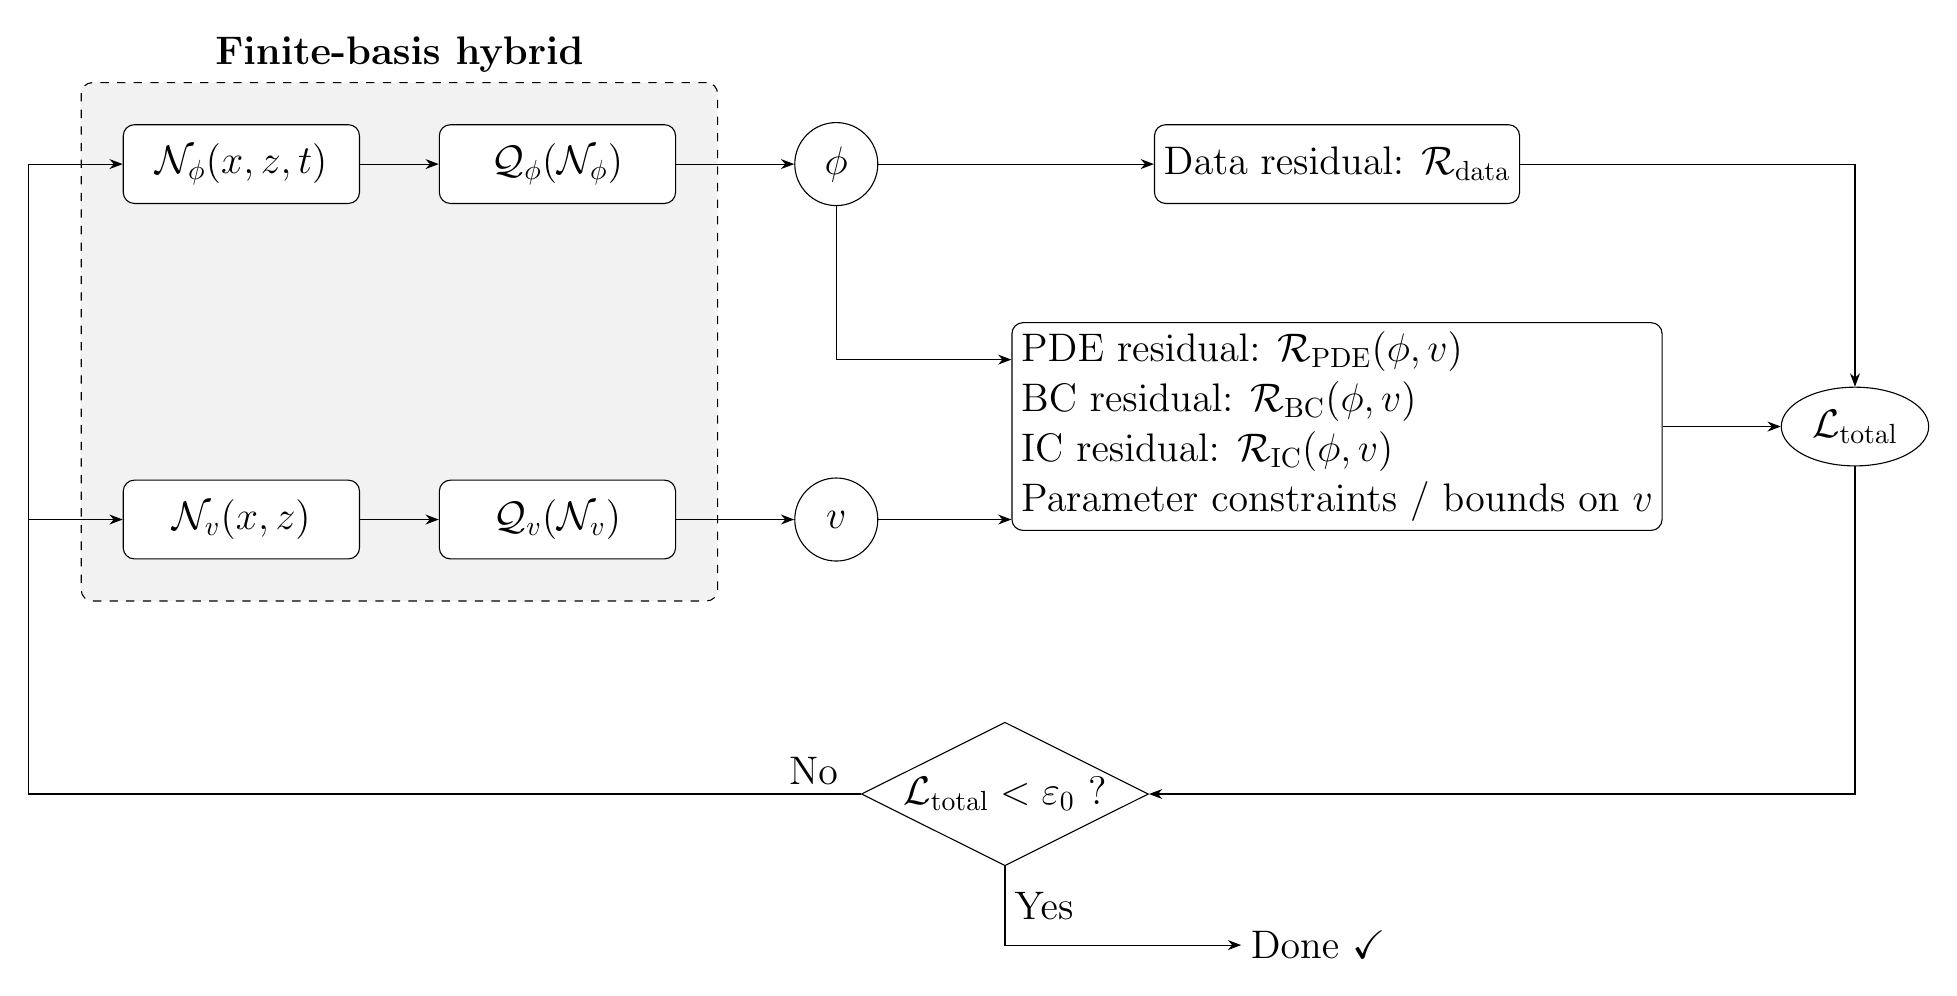
\begin{tikzpicture}[
  >=Stealth,
  font=\Large,
  node distance=2.2cm and 2.4cm,
  box/.style={draw, rounded corners, minimum width=3.0cm, minimum height=1.0cm, align=center, fill=white},
  qbox/.style={box},
  circ/.style={circle, draw, minimum size=30, fill=white},
  loss/.style={ellipse, draw, minimum width=1.8cm, minimum height=1.0cm, align=center, fill=white},
  data/.style={box, minimum width=3.0cm},
  physmain/.style={draw, rounded corners, minimum width=4.0cm, minimum height=2.0cm, align=left, fill=white},
  decision/.style={diamond, draw, aspect=2, minimum width=1.6cm, inner sep=1pt, align=center, fill=white}
]

% --- NODES ---
\node[box] (net1) {$\mathcal{N}_\phi(x, z, t)$};
\node[box, below=3.5cm of net1] (net2) {$\mathcal{N}_v(x,z)$};
\node[qbox, right=1.cm of net1] (qc1) {$\mathcal{Q}_\phi(\mathcal{N}_\phi)$};
\node[qbox, right=1.cm of net2] (qc2) {$\mathcal{Q}_v(\mathcal{N}_v)$};


\node[circ, right=1.5cm of qc1] (phi) {$\phi$};
\node[circ, right=1.5cm of qc2] (cvar) {$v$};
\node[data, right=3.5 cm of phi] (data) {Data residual: $\mathcal{R}_{\mathrm{data}}$};
\node[physmain, below=1.5cm of data] (phys)
{PDE residual: $\mathcal{R}_{\mathrm{PDE}}(\phi,v)$\\
BC residual: $\mathcal{R}_{\mathrm{BC}}(\phi,v)$\\
IC residual: $\mathcal{R}_{\mathrm{IC}}(\phi,v)$\\
Parameter constraints / bounds on $v$};
\node[loss, right=1.5cm of phys] (loss) {$\mathcal{L}_{\mathrm{total}}$};

% --- BACKGROUND BOX ---
\begin{scope}[on background layer]
    \node[draw, dashed, fill=gray!10, rounded corners, inner sep=15pt, 
          fit=(net1) (net2) (qc1) (qc2), label=above:{\textbf{Finite-basis hybrid}}] (hybridbox) {};
\end{scope}

% --- CENTERED DECISION NODE ---
% This calculates the horizontal center between the hybridbox west and loss east
\node[decision] (eps) at ($(hybridbox.west |- 0, -8.0) !0.5! (loss.east |- 0, -8.0)$) {$\mathcal{L}_{\mathrm{total}} < \varepsilon_0$ ?};

% --- CONNECTIONS ---
\draw[->] (net1) -- (qc1);
\draw[->] (net2) -- (qc2);
\draw[->] (qc1) -- (phi);
\draw[->] (qc2) -- (cvar);
\draw[->] (phi) -- (data.west);
\draw[->] (phi) |- ([yshift=0.85cm]phys.west);
\draw[->] (cvar) -- (cvar -| phys.west);
\draw[->] (data.east) -| (loss.north);
\draw[->] (phys.east) -- (loss.west);

% Path to loss
\draw[->] (loss.south) |- (eps.east);

% Feedback loop
\draw[-] (eps.west) -- node[above, pos=0.2] {No} ++(-3cm,0) -| ([xshift=-1.2cm]net2.west);
\draw[->] ([xshift=-1.2cm]net2.west) |- (net1.west);
\draw[->] ([xshift=-1.2cm]net2.west) -- (net2.west);

% Yes path: Down, then Right
\draw[->] (eps.south) |- ++(3cm, -1.0cm) node[right] {Done \checkmark} 
    node[near start, right] {Yes};

\end{tikzpicture}%
}
\caption{Schematic of the finite-basis classical--quantum hybrid architecture, combining classical neural networks and quantum circuits with physics-informed constraints. $\mathcal{N}$ denotes classical networks, $\mathcal{Q}$ quantum circuits, $\phi$ the predicted wavefield, $v$ the inverted velocity, and $\mathcal{R}$ the physics- and data-based residuals.}
\label{fig:hybrid_arch}
\end{figure}

\def\myvdots{\ \vdots\ }
\def\myddots{\ \ddots\ }
\begin{figure}[h]
\centering
\resizebox{0.9\linewidth}{!}{
    \begin{quantikz}
    \lstick{$\ket{q_1}$}
        & \gate{R_y(\beta_1 x_1)}
            \gategroup[5,steps=1,style={dashed, fill=gray!10, rounded corners, inner xsep=2pt},background,
            label style={label position=below,anchor=north,yshift=-0.2cm}]
            {{\textbf{Encoding}}}
        & \gate{R_x(\theta_{1,2})}
            \gategroup[5,steps=7,style={dashed, fill=gray!10, rounded corners, inner xsep=2pt},background,
            label style={label position=below,anchor=north,yshift=-0.2cm}]
            {{\textbf{Repeat $N_{Q}$ times}}}
        & \gate{R_y(\theta_{1,3})}
        & \gate{R_z(\theta_{1,4})}
        & \ctrl{1} & & & & \meter{} \\
    \lstick{$\ket{q_2}$}
        & \gate{R_y(\beta_2 x_2)}
        & \gate{R_x(\theta_{2,2})}
        & \gate{R_y(\theta_{2,3})}
        & \gate{R_z(\theta_{2,4})}
        & \targ{} 
        & \ctrl{1} & & & \meter{}\\
    \lstick{$\ket{q_3}$}
        & \gate{R_y(\beta_3 x_3)}
        & \gate{R_x(\theta_{3,2})}
        & \gate{R_y(\theta_{3,3})}
        & \gate{R_z(\theta_{3,4})}
        & & \targ{}
        & \ctrl{1}
        & & \meter{} \\
    \setwiretype{n} \myvdots
        & \myvdots & \myvdots & \myvdots & \myvdots
        & \myvdots & \myvdots & \myddots & \myddots & \myvdots \\
    \lstick{$\ket{q_n}$}
        & \gate{R_y(\beta_n x_n)}
        & \gate{R_x(\theta_{n,2})}
        & \gate{R_y(\theta_{n,3})}
        & \gate{R_z(\theta_{n,4})}
        & & & & \targ{} & \meter{}
    \end{quantikz}
}
\caption{Multilayer parameterized quantum circuit $\mathcal{Q}$. Each classical input feature $x_i$ is angle-encoded via an $R_y(\beta_i\, x_i)$ rotation (encoding layer, grey), where $\beta_i$ is a trainable scaling parameter. Variational layers of single-qubit rotations $R_x$, $R_y$, $R_z$ followed by a linear CNOT ladder are repeated $N_Q$ times (grey block). Each qubit is measured in the Pauli-$Z$ basis, and the outputs are averaged to yield a scalar in $[-1, 1]$.}
\label{fig:pqc_architecture}
\end{figure}

\subsection{Anomaly benchmark}
\label{sec:results_anomaly}

We adopt the velocity model of Rasht-Behesht et al.~\cite{rahst}: a 2D acoustic domain of $1.15$\,km\,$\times$\,$0.45$\,km containing a localized low-velocity anomaly ($\sim$$2.5$\,km/s within a $\sim$$3.0$\,km/s background). Ground-truth data generated by spectral element method~\newcite{komatitsch1998spectral} forward modelling with a Gaussian source at $(0.35,\,0.19)$\,km; 20 receivers along the right boundary ($x = 1.15$\,km) record $500$\,ms of wavefield displacements. Two early displacement snapshots ($t_0 = 0.100$\,s and $t_1 = 0.115$\,s) and the full seismogram record drive the FBPINN inversion.

Both classical and quantum hybrid models recover the low-velocity anomaly from a homogeneous initial model. Figure~\ref{fig:anomaly}(a--c) shows the true, initial, and inverted velocity models: the anomaly location and amplitude closely match the true model, with residual smoothing along the direction of limited source-receiver illumination that is consistent with the benchmark geometry.

Figure~\ref{fig:anomaly}(d) shows the L1 velocity error as a function of training iteration for the classical FBPINN baseline and the quantum hybrid. The quantum hybrid reaches an L1 error of approximately $2.4\times 10^{-2}$ after $65{,}000$ iterations, already below the classical baseline's L1 error of approximately $2.9\times 10^{-2}$ at $500{,}000$ iterations -- an $\sim$$8\times$ reduction in the number of training steps required to reach comparable inversion accuracy. The quantum hybrid also uses fewer trainable parameters overall ($101{,}812$ vs.\ $151{,}836$ for the classical baseline). We interpret this as improved optimization dynamics from the quantum-hybrid parameterization of the velocity field, rather than a claim of quantum computational advantage: the PQC is simulated classically on GPU (Methods), so the reduction is in optimization iterations, not in quantum-hardware runtime.

To verify that the quantum hybrid's advantage is robust to classical hyperparameter choices, we ran 15 additional classical FBPINN variants spanning velocity-network capacity ($c$-network hidden sizes from $10\!\times\!2$ to $60\!\times\!3$), wavefield-network size ($\phi$-network hidden sizes $16\!\times\!2$ and $64\!\times\!3$), subdomain decomposition ($3\!\times\!2\!\times\!3$ and $8\!\times\!4\!\times\!8$), learning rate ($5\!\times\!10^{-5}$ to $5\!\times\!10^{-4}$), subdomain overlap ($0.35$ and $0.50$), and loss weights. All variants are shown in Figure~\ref{fig:anomaly}d as thin coloured curves and listed in Supplementary Table~S1. None of the 15 classical variants match the quantum hybrid's L1 error at any point through $500{,}000$ iterations. The convergence advantage is therefore not an artefact of a specific classical baseline choice.

\begin{figure}[H]
\centering
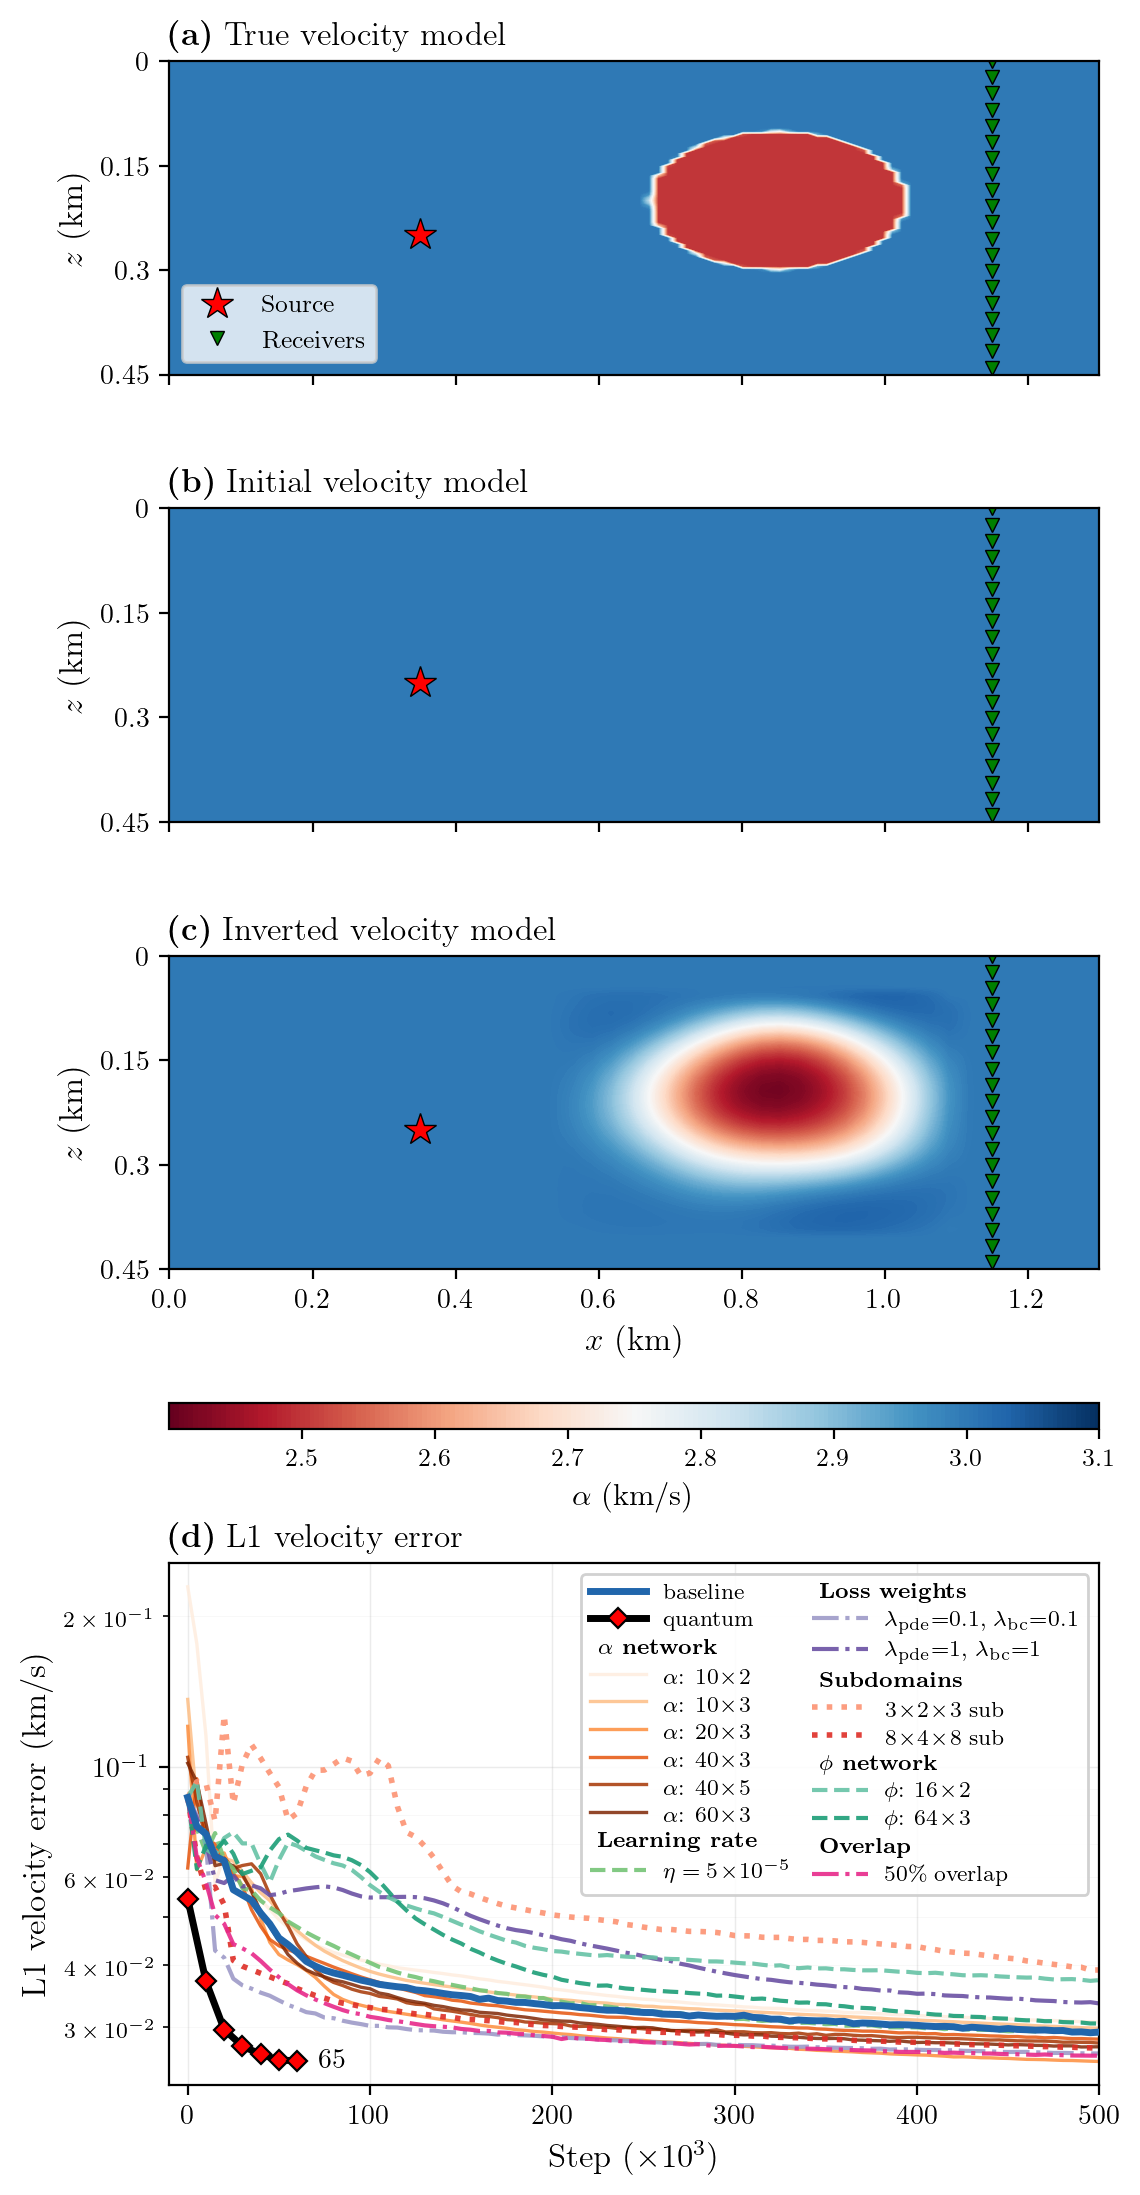
\includegraphics[width=0.6\linewidth]{../results/rasht/plots/l1_and_velocity.png}
\caption{Anomaly benchmark inversion and convergence. (a) True velocity model used for the SPECFEM2D forward simulation, with source (red star) and receiver array (green triangles). (b) Initial homogeneous velocity model. (c) Inverted velocity model from the quantum hybrid FBPINN at $65{,}000$ training iterations. (d) L1 velocity error versus training iteration for the classical FBPINN baseline (blue), the quantum hybrid (red markers labelled 65k), and 15 classical hyperparameter variants (thin coloured lines). The quantum hybrid reaches a lower L1 error than any classical variant in approximately $8\times$ fewer training iterations.}
\label{fig:anomaly}
\end{figure}

\subsection{Checkerboard benchmark}
\label{sec:results_checkerboard}

To assess resolution characteristics, we also invert a checkerboard velocity model: a $3\times 3$ grid of alternating $\pm$$0.4$\,km/s perturbations on a $3.0$\,km/s background, embedded in the same domain and source-receiver geometry as the anomaly benchmark (Figure~\ref{fig:checkerboard_inversion}a). The classical FBPINN recovers the checkerboard structure after $2\times 10^{6}$ training iterations (Figure~\ref{fig:checkerboard_inversion}b), with resolution progressively degrading for blocks located further from the receiver array -- consistent with the limited angular coverage provided by a single source and a one-sided receiver line. A quantum hybrid experiment on this benchmark is in progress and will be reported in a revised version of this work; the quantitative convergence comparison of the anomaly benchmark therefore rests on the anomaly benchmark alone.

\begin{figure}[h]
\centering
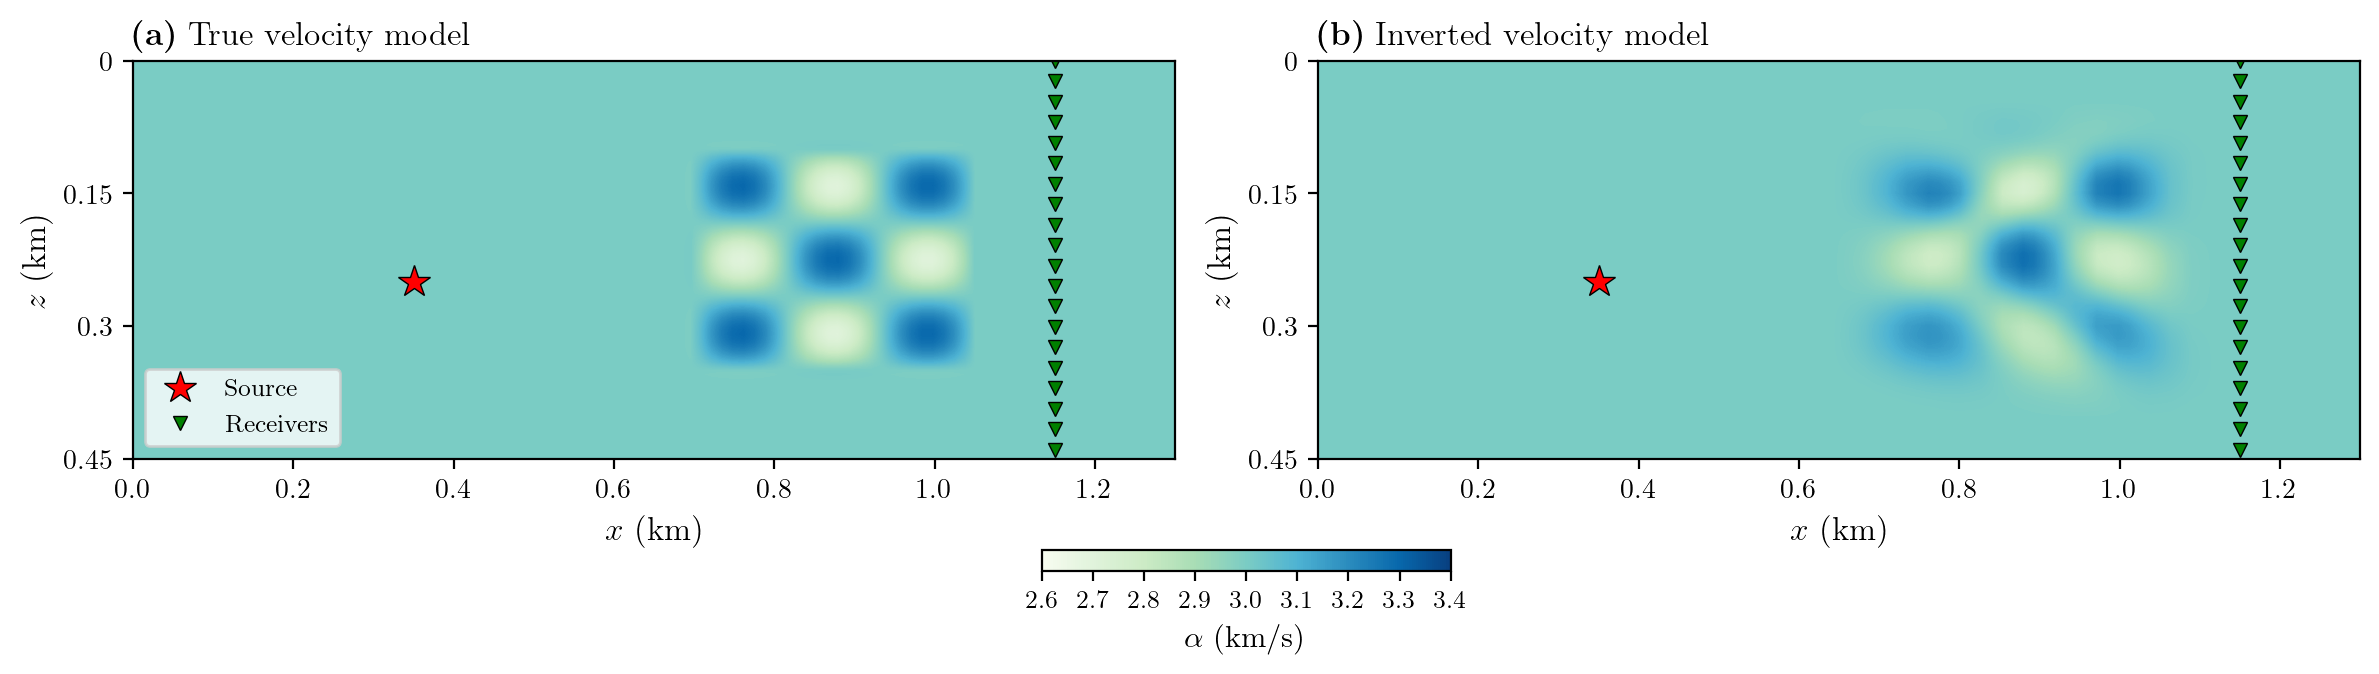
\includegraphics[width=\linewidth]{../results/checkerboard/plots/true_and_inverted.png}
\caption{Checkerboard benchmark inversion. (a) True velocity model: a $3\times 3$ checkerboard of alternating $\pm$$0.4$\,km/s perturbations on a $3.0$\,km/s background, with source (red star) and receiver array (green triangles). (b) Inverted velocity model from the classical FBPINN at $2\times 10^{6}$ training iterations. Quantum hybrid results for this benchmark are forthcoming.}
\label{fig:checkerboard_inversion}
\end{figure}


\section{Discussion}\label{sec:discussion}

The quantum hybrid velocity network reaches a lower L1 velocity error than the classical FBPINN baseline and all 15 classical hyperparameter variants in approximately $8\times$ fewer training iterations, while using $\sim$$33$\% fewer trainable parameters. We attribute this to three properties of the classical-to-PQC pipeline~\newcite{cerezo2021variational}. First, despite its smaller parameter count, the PQC operates in an exponentially large Hilbert space~\newcite{havlicek2019supervised,huang2021power}: an $n$-qubit statevector has $2^n$ complex amplitudes (for $n=4$, a $16$-dimensional complex space, i.e.\ $32$ real degrees of freedom per evaluation), and the measured expectation value
\begin{equation}
    f(\mathbf{x};\boldsymbol{\beta},\boldsymbol{\theta}) = \frac{1}{n}\sum_{i=0}^{n-1} \langle\psi(\mathbf{x};\boldsymbol{\beta},\boldsymbol{\theta})|\,Z_i\,|\psi(\mathbf{x};\boldsymbol{\beta},\boldsymbol{\theta})\rangle
\end{equation}
is a nonlinear function of all variational angles acting jointly on this high-dimensional representation. A classical MLP with a comparable parameter count operates in a much smaller latent space and must spend its parameters on both feature construction and output generation. Second, angle encoding endows the PQC output with a specific finite-frequency Fourier structure~\newcite{schuld2021effect},
\begin{equation}
    f(\mathbf{x}) = \sum_{\boldsymbol{\omega}\in\Omega} c_{\boldsymbol{\omega}}(\boldsymbol{\theta})\, e^{i\,\boldsymbol{\omega}\cdot(\boldsymbol{\beta}\odot\mathbf{x})},
\end{equation}
in which the trainable angles control the Fourier coefficients $c_{\boldsymbol{\omega}}$ while the accessible frequency set $\Omega$ is fixed by the eigenvalues of the encoding generators. This built-in spectral prior may match smooth, spatially-correlated velocity fields more efficiently than an unconstrained tanh MLP, which has no such structure by default. Third, the PQC output is bounded to $[-1, 1]$ by construction, which hard-codes a range constraint on the velocity perturbation (equation~\ref{eq:velocity_output}) and removes an avenue for early training to wander into pathological high-amplitude solutions; entangling CNOT gates additionally introduce non-separable correlations between the spatial inputs that a product-structured MLP only recovers through repeated tensor contractions. The robustness of the advantage across classical hyperparameter choices (Figure~\ref{fig:anomaly}d) argues against an unlucky baseline, though we emphasize that these gains are in optimization iterations on classically-simulated circuits and do not constitute a quantum computational advantage.

Our work complements recent hybrid quantum-PINN studies in other PDE-constrained settings. Leong et al.~\cite{LEONG2025106782} benchmarked hybrid quantum PINNs for high-speed compressible flow, finding competitive accuracy at reduced parameter cost compared with classical PINNs. Berger et al.~\cite{Berger2025} introduced trainable-embedding quantum PINNs for nonlinear PDEs including the Navier-Stokes equations, again observing efficiency gains at matched parameter count. The present work differs in two ways. First, we target a coupled forward--inverse problem (waveform inversion) rather than a pure forward PDE; the velocity field is learned jointly with the wavefield. Second, we integrate the PQC within a domain-decomposed FBPINN~\cite{Moseley2023}, extending the PINN-based FWI formulation of Rasht-Behesht et al.~\cite{rahst} to handle larger and higher-frequency inversion problems via overlapping subdomain networks.

Several limitations should be noted. (i) The present experiments are two-dimensional and acoustic. Extending to three-dimensional elastic inversion is the natural next step but is constrained by the $\mathcal{O}(2^n)$ memory cost of statevector simulation as qubit counts grow. Scaling to larger circuits on real hardware further raises the concern of barren plateaus -- vanishingly small gradients in high-depth parameterized circuits~\newcite{mcclean2018barren} -- which would require careful initialization and ansatz choice. (ii) Inversions use a single source; production FWI pipelines incorporate tens to thousands of sources with different illuminations, and PINN-based FWI in particular is known to be sensitive to loss-landscape pathologies under data sparsity~\newcite{krishnapriyan2021failure}. (iii) The quantum circuit is simulated classically. On real NISQ hardware, gradients would be computed via the parameter-shift rule (two circuit evaluations per parameter), and device noise could erode the iteration-level advantage observed here. (iv) The quantum hybrid has so far been validated on the anomaly benchmark only; a matched quantum run on the checkerboard benchmark is in progress.

Looking forward, the small qubit counts used here ($n=4$, $L=2$) are compatible with near-term quantum hardware, which suggests that genuine hardware demonstrations are feasible once noise-mitigation techniques reach sufficient maturity. Systematic studies at matched parameter counts across circuit depths and widths would clarify how the convergence advantage scales with quantum-circuit capacity. Beyond geophysics, the framework is directly applicable to any wave-based inverse problem expressible as a physics-informed learning task -- including medical ultrasound tomography~\cite{10.1121/1.3699240,Sandhu_2015}, photoacoustic imaging~\cite{Wang2016}, and non-destructive evaluation~\cite{7422116} -- and we expect the same convergence benefits to transfer to those settings.

\section{Methods}\label{sec:method}

\subsection{Acoustic wave equation}
\label{sec:methods_wave}

We consider two-dimensional acoustic wave propagation in a heterogeneous medium with spatially varying wave speed $c(\mathbf{x})$ and constant density. With no explicit source injection, the governing equation is the source-free acoustic wave equation,
\begin{equation}
\frac{\partial^{2} u(\mathbf{x},t)}{\partial t^{2}}
= c^{2}(\mathbf{x})\,\nabla^{2} u(\mathbf{x},t),
\label{eq:acoustic_wave}
\end{equation}
where $u(\mathbf{x},t)$ is a scalar potential whose spatial derivatives $(\partial u/\partial x,\, \partial u/\partial z)$ give the two components of the displacement field. Wave propagation is initiated by prescribing the wavefield at two closely-spaced instants, $t_0 = 0.100$\,s and $t_1 = 0.115$\,s, using snapshots of the displacement field taken from a spectral-element simulation; both snapshots are imposed as soft constraints in the loss function. A free-stress boundary condition (vanishing pressure Laplacian) is enforced on the top surface of the physical domain. This formulation provides a well-posed initial-boundary-value problem without requiring an explicit source time function.

\subsection{Finite-basis physics-informed neural network}
\label{sec:methods_fbpinn}

Physics-informed neural networks (PINNs)~\cite{RAISSI2019686} approximate solutions of partial differential equations by a neural network $u_\theta(\mathbf{x})$ and train $\theta$ to minimize the PDE residual at a set of collocation points $\{\mathbf{x}_i\}_{i=1}^{N}$ drawn from the domain. Writing the governing PDE in residual form $\mathcal{N}[u](\mathbf{x}) = 0$, the PDE loss is
\begin{equation}
    \mathcal{L}_\text{PDE}
    = \frac{1}{N} \sum_{i=1}^{N}
    \left| \mathcal{N}[u_\theta(\mathbf{x}_i)] \right|^{2},
\end{equation}
with spatial and temporal derivatives computed by automatic differentiation of the network with respect to its inputs. Boundary conditions, initial conditions, and observational data are added as additional weighted loss terms (the full composite loss used for FWI is given in the Hybrid architecture subsection below). Standard PINNs, however, are known to suffer from spectral bias -- a tendency to learn low-frequency features before high-frequency ones -- which severely limits their effectiveness in multi-scale wave problems such as FWI, where both the velocity field and the wavefield exhibit sharp transitions and oscillatory structure.

To overcome this limitation, we adopt the Finite-Basis Physics-Informed Neural Network (FBPINN) framework of \citet{Moseley2023}. The global domain $\Omega$ is partitioned into $K$ overlapping rectangular subdomains $\{\Omega_k\}$, each equipped with an independent neural network $u_{\theta_k}(\mathbf{x})$. The global solution is reconstructed as a partition-of-unity sum,
\begin{equation}
    u(\mathbf{x}) = \sum_{k=1}^{K} w_k(\mathbf{x})\, u_{\theta_k}(\mathbf{x}),
\end{equation}
where the window functions $w_k$ are smooth cosine bumps supported on $\Omega_k$ with $\sum_k w_k(\mathbf{x}) = 1$ for all $\mathbf{x} \in \Omega$. Each local network only needs to represent the solution's behaviour on its own subdomain, with two consequences: (i) the local frequency content each network must learn is bounded by the subdomain size, alleviating spectral bias; and (ii) training is embarrassingly parallel across subdomains, enabling batched evaluation via JAX's \texttt{vmap}. The physics-informed loss is evaluated on the reconstructed global solution, so gradients flow through the window-weighted sum back to the individual subdomain networks.

For the wavefield $\phi(x,z,t)$ we use a three-dimensional subdomain decomposition $(n_x, n_z, n_t)$, $5\!\times\!3\!\times\!5$ in the anomaly baseline with subdomain overlap $0.35$. The velocity network $c(x,z)$ is not decomposed -- it is a single global network -- since the velocity field typically varies more smoothly than the wavefield and does not require local representation.

\subsection{Parameterized quantum circuits}
\label{sec:methods_pqc}

This section introduces the quantum computing concepts required to
understand the hybrid classical--quantum architecture presented in
the Hybrid architecture subsection of Methods.

\subsubsection{Qubits and quantum states}

The fundamental unit of quantum information is the qubit, a
two-level quantum system whose state is represented by a unit vector in
$\mathbb{C}^2$.  In the computational basis $\{|0\rangle, |1\rangle\}$,
an arbitrary single-qubit state is written as
\begin{equation}
  |\psi\rangle = \alpha\,|0\rangle + \beta\,|1\rangle, \qquad
  |\alpha|^2 + |\beta|^2 = 1,
\end{equation}
where $\alpha, \beta \in \mathbb{C}$ are probability amplitudes.
Geometrically, the state of a single qubit can be visualised as a point
on the Bloch sphere, parameterised by polar and azimuthal angles.  An
$n$-qubit register is described by a statevector in
$\mathbb{C}^{2^n}$,
\begin{equation}
  |\psi\rangle = \sum_{k=0}^{2^n - 1} \alpha_k\,|k\rangle, \qquad
  \sum_{k=0}^{2^n - 1} |\alpha_k|^2 = 1,
\end{equation}
where $|k\rangle$ denotes the $k$-th computational basis state.  The
exponential growth of the Hilbert space dimension with qubit count
underlies both the potential computational advantage of quantum systems
and the cost of their classical simulation.

\subsubsection{Quantum gates}

Quantum computation proceeds by applying quantum gates -- unitary transformations that evolve the statevector while preserving its norm. The circuit used in this work employs two kinds of gate.

The single-qubit rotations $R_x(\theta)$, $R_y(\theta)$, $R_z(\theta)$ are parameterized unitaries
\begin{equation}
  R_k(\theta) = e^{-i\theta\,\sigma_k/2}, \qquad k \in \{x,y,z\},
\end{equation}
where $\sigma_k$ are the Pauli matrices. Written explicitly,
\begin{equation}
  R_x(\theta) =
  \begin{pmatrix} \cos\tfrac{\theta}{2} & -i\sin\tfrac{\theta}{2} \\
  -i\sin\tfrac{\theta}{2} & \cos\tfrac{\theta}{2} \end{pmatrix},
\quad
  R_y(\theta) =
  \begin{pmatrix} \cos\tfrac{\theta}{2} & -\sin\tfrac{\theta}{2} \\
  \sin\tfrac{\theta}{2} & \cos\tfrac{\theta}{2} \end{pmatrix},
\quad
  R_z(\theta) =
  \begin{pmatrix} e^{-i\theta/2} & 0 \\
  0 & e^{i\theta/2} \end{pmatrix}.
\end{equation}
Each gate rotates the single-qubit state by angle $\theta$ about the corresponding axis of the Bloch sphere, and the composition $R_z(\theta_3)\,R_y(\theta_2)\,R_x(\theta_1)$ is a general single-qubit unitary with three independent parameters, capable of mapping the initial state to any point on the Bloch sphere.

The entangling gate is the controlled-NOT (CNOT), a two-qubit unitary that flips the target qubit if and only if the control qubit is in state $|1\rangle$:
\begin{equation}
  \mathrm{CNOT} =
  \begin{pmatrix} 1 & 0 & 0 & 0 \\
                  0 & 1 & 0 & 0 \\
                  0 & 0 & 0 & 1 \\
                  0 & 0 & 1 & 0 \end{pmatrix}.
\end{equation}
CNOT is the sole multi-qubit gate used in our circuit and the sole source of entanglement -- correlations between qubits that have no classical analogue -- which enables the PQC to represent functions of multiple input features that cannot be factorized across individual qubits.

\subsubsection{PQC ansatz}
\label{sec:circuit_architecture}

A parameterised quantum circuit (PQC)~\cite{benedetti2019parameterized}, also referred to as a variational quantum circuit, applies a trainable unitary $U(\boldsymbol{\theta})$ to the initial state $|0\rangle^{\otimes n}$ and returns a scalar expectation value of a Hermitian observable, yielding a smooth, differentiable function of $\boldsymbol{\theta}$ that acts as a trainable function approximator. Its expressibility depends on the circuit depth, qubit connectivity, and gate set~\cite{sim2019expressibility}.

The PQC employed in this work (Fig.~\ref{fig:pqc_architecture}) operates on $n$ qubits with $L$ variational layers and consists of three stages:

\begin{enumerate}
  \item \emph{Data embedding layer.} Starting from $|0\rangle^{\otimes n}$, each qubit $i$ receives an $R_y(\beta_i\, x_i)$ rotation (angle encoding~\cite{schuld2021machine}) that encodes the $i$-th component of the classical input vector $\mathbf{x} \in \mathbb{R}^n$, scaled by a trainable basis parameter $\beta_i$:
    \begin{equation}
      |\psi_0\rangle = \bigotimes_{i=0}^{n-1} R_y(\beta_i\, x_i)\,|0\rangle.
    \end{equation}

  \item \emph{Variational layers.} Each of $L$ layers $l = 1, \ldots, L$ applies (i) a general single-qubit rotation $R_z(\theta^{(3)}_{l,i})\, R_y(\theta^{(2)}_{l,i})\, R_x(\theta^{(1)}_{l,i})$ to every qubit $i$, introducing $3n$ trainable parameters per layer, followed by (ii) a linear CNOT ladder $\text{CNOT}(i, i{+}1)$ for $i = 0, \ldots, n{-}2$ entangling neighbouring qubits. The total number of trainable gate parameters is $3nL$, plus $n$ basis parameters from the embedding layer.

  \item \emph{Measurement layer.} The Pauli-$Z$ expectation values $\langle Z_i \rangle$ on each qubit are averaged to produce a single scalar output
    \begin{equation}
      f(\mathbf{x}, \boldsymbol{\beta}, \boldsymbol{\theta})
      = \frac{1}{n} \sum_{i=0}^{n-1} \langle\psi|\, Z_i \,|\psi\rangle
      \;\in [-1,\, 1].
      \label{eq:pqc_output}
    \end{equation}
    The bounded output is rescaled by trainable output weights and biases in the surrounding classical layers.
\end{enumerate}

\subsection{JAX-based statevector simulator}
\label{sec:methods_statevector}

We implement the PQC as a lightweight statevector simulator in JAX~\citep{jax2018github} rather than relying on an external framework such as PennyLane~\citep{bergholm2022pennylaneautomaticdifferentiationhybrid} or Qiskit~\citep{javadiabhari2024quantumcomputingqiskit}. The simulator represents the quantum state as a $2^n$-dimensional complex vector and applies gate operations via tensor contractions: single-qubit rotation gates ($R_x$, $R_y$, $R_z$) are constructed as $2\!\times\!2$ unitary matrices and applied with \texttt{jnp.tensordot} on the reshaped state tensor, and CNOT gates are realised through index permutation and conditional flipping on the control-target subspace. Expectation values are computed analytically from the statevector amplitudes, without stochastic sampling, and are mathematically equivalent to PennyLane's \texttt{default.qubit} simulator: both perform exact statevector evolution under the same unitary transformations and Born-rule probabilities.

On near-term quantum hardware, gradients of PQC outputs with respect to gate parameters are typically computed via the parameter-shift rule~\newcite{mitarai2018quantum,schuld2019evaluating}, which evaluates the circuit at two shifted parameter values per gate and therefore requires $2p$ circuit evaluations per gradient for a circuit with $p$ parameters. In classical statevector simulation, each gate application is already a standard differentiable operation, so embedding the circuit in JAX offers two concrete advantages. First, \texttt{jax.grad} and \texttt{jax.jvp} backpropagate through the full hybrid pipeline -- classical PINN layers, quantum circuit, and loss function -- without parameter-shift rules or cross-framework bridging. Second, the entire training loop can be compiled into a single optimized XLA program via \texttt{jax.jit}, eliminating Python-level dispatch and framework-bridging overhead. The trade-off is that statevector simulation scales as $\mathcal{O}(2^n)$ in memory and $\mathcal{O}(L\,n\,2^n)$ in computation, limiting the approach to moderate qubit counts; for the circuit sizes used here ($n \leq 8$, $L \leq 6$), this cost is negligible compared with the classical network and loss evaluation. We verify numerical correctness by comparing parameter gradients $\partial f/\partial\boldsymbol{\theta}$ against PennyLane's \texttt{default.qubit} backend~\newcite{bergholm2018pennylane} across eight circuit configurations (2--8 qubits, 1--6 layers); the maximum absolute deviation is below $2\times 10^{-7}$, consistent with \texttt{float32} machine precision (Supplementary Fig.~S1).

\subsection{Hybrid quantum-classical architecture}\label{sec:hybrid_network}

The hybrid architecture (Figure~\ref{fig:hybrid_arch}) couples two neural networks with physics-informed constraints: a wavefield network $\phi(x,z,t)$, decomposed across subdomains as described in \S\ref{sec:methods_fbpinn}, and a velocity network $c(x,z)$, which is a single global network. In the classical baseline, both networks are fully-connected tanh networks. In the quantum hybrid, both networks are classical-to-quantum pipelines.

Each classical-to-quantum pipeline has the form
\begin{equation}
    g(\mathbf{x}) = w_\text{out}\, \mathcal{Q}\!\left(\mathcal{N}(\mathbf{x}; \theta_c); \boldsymbol{\beta}, \boldsymbol{\theta}_q\right) + b_\text{out},
\end{equation}
where $\mathcal{N}$ is a classical fully-connected tanh sub-network that maps $\mathbf{x}$ to an $n$-dimensional latent vector matched to the number of qubits, $\mathcal{Q}$ is the PQC of \S\ref{sec:methods_pqc} (which returns a scalar in $[-1,1]$), and $(w_\text{out}, b_\text{out})$ are learnable output weights. For the anomaly benchmark experiments we use $n = 4$ qubits and $L = 2$ variational layers in both networks. The velocity network output is further mapped to physical velocity units via
\begin{equation}
    c(x,z) = c_\text{bg} + A\, \tanh\!\big(g(x,z)\big) \cdot m(x,z),
    \label{eq:velocity_output}
\end{equation}
with background velocity $c_\text{bg} = 3.0$\,km/s, amplitude $A = 2.0$\,km/s, and a smooth spatial mask $m(x,z) \in [0,1]$ (the product of four logistic cutoffs) that confines the velocity perturbation to the interior of the physical domain. This construction hard-codes physical bounds ($|\alpha - c_\text{bg}| \leq A$) and zero perturbation at the domain edges, acting as a mild regularization of the inverse problem.

The full training objective is
\begin{equation}
\mathcal{L}_\text{total}
= \lambda_\text{data}\,\mathcal{L}_\text{data}(\phi)
+ \lambda_\text{PDE}\,\mathcal{L}_\text{PDE}(\phi, c)
+ \lambda_\text{BC}\,\mathcal{L}_\text{BC}(\phi)
+ \lambda_\text{IC}\,\mathcal{L}_\text{IC}(\phi),
\end{equation}
where $\mathcal{L}_\text{data}$ is the seismogram misfit between the predicted and observed displacement fields at the receiver locations, $\mathcal{L}_\text{PDE}$ enforces the source-free acoustic wave equation~(\ref{eq:acoustic_wave}) via automatic differentiation, and $\mathcal{L}_\text{IC}, \mathcal{L}_\text{BC}$ are the snapshot-based initial-condition and free-stress boundary-condition constraints. All parameters -- classical FC weights, embedding scales $\boldsymbol{\beta}$, variational angles $\boldsymbol{\theta}_q$, and output scalings -- are optimized jointly by Adam gradient descent through the full differentiable pipeline.

\subsection{Training setup}
\label{sec:methods_training}

All training uses the Adam optimizer at learning rate $10^{-4}$ (baseline; see Supplementary Table~S1 for variants). Each training step draws a collocation batch from the subdomains of shape $(n_x, n_z, n_t) = (40,40,25)$ per step ($40{,}000$ PDE collocation points in total), together with $40\!\times\!40 = 1{,}600$ points per displacement snapshot for the two initial-condition constraints, $\sim$$1{,}000$ seismogram observations (20 receivers subsampled every 100 SPECFEM timesteps), and $5{,}000$ randomly-sampled boundary-condition points on the top surface. The composite loss uses fixed weights $\lambda_\text{PDE} = 0.1$, $\lambda_\text{IC} = 1.0$ (applied equally to the two snapshot constraints), $\lambda_\text{data} = 1.0$ (seismogram), and $\lambda_\text{BC} = 0.1$. The classical baseline is trained for $500{,}000$ iterations; the quantum hybrid is trained for $65{,}000$ iterations, at which point it has already surpassed the classical baseline's $500{,}000$-step L1 velocity error.

Training uses JAX's \texttt{jit} and \texttt{vmap} transformations to compile the update step into a single XLA program and batch evaluation over subdomains. The complete update step -- classical-network forward/backward passes, PQC statevector evolution, Jacobian computation via chained forward-mode \texttt{jvp}, and the composite loss -- executes as a single GPU kernel. All experiments were performed on a single NVIDIA GeForce RTX 5090 GPU with \texttt{float64} precision. For the quantum hybrid, the statevector footprint is negligible: the 4-qubit PQC requires only $2^4 = 16$ complex amplitudes per forward pass, so memory cost is dominated by the classical wavefield subdomain networks.

\subsection{Data}
\label{sec:methods_data}

Synthetic seismic data for both benchmarks were generated with SPECFEM2D~\newcite{komatitsch1998spectral}, a spectral-element forward solver. Configuration files and receiver layouts are distributed with the project repository (\texttt{data/rasht/specfem/} and \texttt{data/checkerboard/specfem/}).

\textit{Anomaly benchmark.}
The physical domain is $1.15$\,km $\times\ 0.45$\,km after removing a ten-element absorbing boundary layer. A single seismic source at $(0.35, 0.19)$\,km emits a Gaussian wavelet in the SPECFEM forward run; 20 receivers are deployed vertically along $x = 1.15$\,km at $\sim$$22.5$\,m spacing. Recording length is $500$\,ms ($10{,}000$ SPECFEM timesteps at $\Delta t_\text{spec} = 5\times 10^{-5}$\,s), subsampled every $100$ timesteps for the seismogram loss. Two wavefield snapshots at $t_0 = 0.100$\,s and $t_1 = 0.115$\,s (SPECFEM timesteps 2000 and 2300) are used as initial-condition constraints for the FBPINN training. Spatial coordinates are scaled by $L_x = L_z = 3$\,km in all training computations.

\textit{Checkerboard benchmark.}
Same domain geometry, source position, and receiver layout as the anomaly benchmark, but with a $3\!\times\!3$ checkerboard velocity pattern of alternating $\pm$$0.4$\,km/s perturbations on a $3.0$\,km/s background, spatially confined to $[0.70, 1.05]\,\text{km} \times [0.10, 0.30]\,\text{km}$.


\section{Conclusions}

We introduced a hybrid quantum-classical FBPINN for acoustic FWI, integrating a parameterized quantum circuit into the velocity network within a domain-decomposed physics-informed framework. The approach is implemented as an end-to-end differentiable JAX program, avoiding parameter-shift-rule overhead and enabling efficient joint optimization of classical PINN parameters and quantum circuit angles. On the anomaly benchmark, the hybrid model converges in $\sim$$8\times$ fewer training iterations than a classical FBPINN baseline -- and than 15 classical hyperparameter variants -- while using $\sim$$33$\% fewer trainable parameters. We emphasize that these gains are in optimization iteration count on classically-simulated circuits, and do not constitute a claim of quantum computational advantage. Key limitations include reliance on classical statevector simulation, a two-dimensional acoustic setup, and a single-source configuration; extension to elastic, three-dimensional, and multi-source inversion, as well as validation on near-term quantum hardware, are the natural next steps. The framework generalizes beyond geophysics to any wave-based inverse problem amenable to physics-informed learning.


\section*{Data availability}
The synthetic seismic data used in this study were generated with SPECFEM2D~\newcite{komatitsch1998spectral} and are available in the project repository at \url{https://github.com/x-repos/quFWI} under \texttt{data/rasht/} and \texttt{data/checkerboard/}.

\section*{Code availability}
The JAX-based quantum simulator and \texttt{quFWI} framework presented here are available at \url{https://github.com/x-repos/quFWI}. Our implementation builds upon the FBPINNs framework~\cite{Moseley2023} (\url{https://github.com/benmoseley/FBPINNs}) with the PINN-based FWI formulation of Rasht-Behesht et al.~\cite{rahst} (\url{https://github.com/maziarash/PINN-FWI}).

\section*{Acknowledgments}
We would like to thank the Reservoir Characterization Project (RCP), Colorado School of Mines, for the financial support.

\section*{Author contributions}
% FILL: author contribution statement.

\section*{Conflicts of interest}
The authors declare no competing interests.

\bibliographystyle{unsrtnat}
\bibliography{refs}

\end{document}
